%\renewcommand{\theequation}{\theenumi}
%\begin{enumerate}[label=\arabic*.,ref=\thesection.\theenumi]
%\numberwithin{equation}{enumi}
% \renewcommand{\thefigure}{\theenumi}
% \numberwithin{figure}{enumi}
%
\item Draw Fig. \ref{fig:tri_right_angle} for $a = 4, c =3$.
\label{const:tri_right_angle}
%
\begin{figure}[!ht]
\centering
\resizebox{\columnwidth}{!}{\input{./figs/triangle/tri_right_angle.tex}}
\caption{Right Angled Triangle}
\label{fig:tri_right_angle}	
\end{figure}
\\
\solution The vertices of $\triangle ABC$ are 
\begin{align}
\vec{A} = \myvec{0\\c} = \myvec{0\\3}, \vec{B} = \myvec{0\\0}, \vec{C} = \myvec{a\\0}=\myvec{4\\0}
\end{align}
%
The python code for  Fig. \ref{fig:tri_right_angle} is
\begin{lstlisting}
codes/triangle/tri_right_angle.py
\end{lstlisting}
%
and the equivalent latex-tikz code is
%
\begin{lstlisting}
figs/triangle/tri_right_angle.tex
\end{lstlisting}
%
The above latex code can be compiled as a standalone document as
%
\begin{lstlisting}
figs/triangle/tri_right_angle_alone.tex
\end{lstlisting}
%

\item Draw Fig. \ref{fig:tri_polar} for $a = 4, c =3$.
\label{const:tri_polar}
%
\\
\solution 
 The vertex  $\vec{A}$ can  be expressed  in {\em polar coordinate form} as
%\label{prob:tri_polar}
%
\begin{align}
\vec{A} = b\myvec{\cos \theta\\  \sin \theta} 
\end{align}
%
where
\begin{align}
b = \sqrt{a^2+c^2} = 5, \tan \theta = \frac{3}{4}
\end{align}
%The vertices of $\triangle ABC$ are 
%\begin{align}
%\vec{A} = \myvec{a\\c} = \myvec{4\\3}, \vec{B} = \myvec{a\\0}  = \myvec{4\\0}, \vec{C} = \myvec{0\\0}.
%\end{align}
%
The python code for  Fig. \ref{fig:tri_polar} is
\begin{lstlisting}
codes/triangle/tri_polar.py
\end{lstlisting}
%
and the equivalent latex-tikz code is
%
\begin{lstlisting}
figs/triangle/tri_polar.tex
\end{lstlisting}
\begin{figure}[!ht]
\centering
\resizebox{\columnwidth}{!}{\input{./figs/triangle/tri_polar.tex}}
\caption{Right Angled Triangle}
\label{fig:tri_polar}	
\end{figure}
%
\item Draw Fig. \ref{fig:tri_sss} with $a=6$, $b=5$  and $c=4$.  
\label{const:tri_sss}
\begin{figure}[!ht]
	\begin{center}
			\resizebox{\columnwidth}{!}{\input{./figs/triangle/tri_sss.tex}}
	\end{center}
	\caption{}
	\label{fig:tri_sss}	
\end{figure}
\\
\solution Let the vertices of  $\triangle ABC$ and $\vec{D}$ be 
\begin{align}
\label{eq:tri_basic}
\vec{A} = \myvec{p\\q}, \vec{B} = \myvec{0\\0}, \vec{C} = \myvec{a\\0}, \vec{D} = \myvec{p\\0}
\end{align}
%

Then
\begin{align}
\label{eq:c_tricoord}
AB &= \norm{\vec{A}-\vec{B}}^2 = \norm{\vec{A}}^2  = c^2 \quad \because \vec{B} = \vec{0}
\\
\label{eq:a_tricoord}
BC &= \norm{\vec{C}-\vec{B}}^2 = \norm{\vec{C}}^2  = a^2
\\
AC &= \norm{\vec{A}-\vec{C}}^2 =    b^2
\label{eq:b_tricoord}
\end{align}
%
From \eqref{eq:b_tricoord},
\begin{align}
b^2 &=\norm{\vec{A}-\vec{C}}^2 = \norm{\vec{A}-\vec{C}}^T\norm{\vec{A}-\vec{C}}  
\\
&= \vec{A}^T\vec{A}+\vec{C}^T\vec{C}-\vec{A}^T\vec{C} - \vec{C}^T\vec{A} 
\\
&= \norm{\vec{A}}^2 + \norm{\vec{C}}^2 - 2\vec{A}^T\vec{C} \quad \brak{\because \vec{A}^T\vec{C} = \vec{C}^T\vec{A} } 
\label{eq:tri_const_norm_ac}
\\
&= a^2+c^2-2ap
\end{align}
%
yielding
\begin{align}
p&= \frac{a^2+c^2-b^2}{2a}
\end{align}
%
From \eqref{eq:c_tricoord}, 
\begin{align}
\norm{\vec{A}}^2 &= c^2 = p^2+q^2
\\
\implies q&= \pm \sqrt{c^2-p^2}
\end{align}
%
The python code for  Fig. \ref{fig:tri_sss} is
\begin{lstlisting}
codes/triangle/tri_sss.py
\end{lstlisting}
%
and the equivalent latex-tikz code is
%
\begin{lstlisting}
figs/triangle/tri_sss.tex
\end{lstlisting}

\item Construct a triangle of sides $a=4$, $b=5$  and $c=6$.  
\\
\solution

Let the given Matrix be
\begin{equation}
\vec{A} = \myvec{3&5\\1&1}
\end{equation}
Transposing the above matrix gives,
\begin{equation}
\vec{A}^{\top} = \myvec{3&1\\5&1}
\end{equation}
Now, for Symmetric and Skew Symmetric Matrix,
\begin{align}
    \vec{B} &= \frac{\vec{A} + \vec{A}^{\top}}{2} = \myvec{3&3\\3&1} \\
    &= \vec{B}^{\top}
\end{align}
Also,
\begin{align}
    \vec{C} &= \frac{\vec{A} - \vec{A}^{\top}}{2} = \myvec{0&2\\-2&0} \\
    &= -\vec{C}^{\top}
\end{align}

Hence, $\vec{B}$ is a Symmetric Matrix and $\vec{C}$ is a Skew Symmetric Matrix and $\vec{B} + \vec{C} = \vec{A}$.
\begin{align}
    \therefore \myvec{3&5\\1&1} = \myvec{3&3\\3&1} + \myvec{0&2\\-2&0}  
\end{align}





\item Construct an isosceles triangle whose base is $a=8$cm and altitude $AD=h=4$cm 
\\
\solution

Let the given Matrix be
\begin{equation}
\vec{A} = \myvec{3&5\\1&1}
\end{equation}
Transposing the above matrix gives,
\begin{equation}
\vec{A}^{\top} = \myvec{3&1\\5&1}
\end{equation}
Now, for Symmetric and Skew Symmetric Matrix,
\begin{align}
    \vec{B} &= \frac{\vec{A} + \vec{A}^{\top}}{2} = \myvec{3&3\\3&1} \\
    &= \vec{B}^{\top}
\end{align}
Also,
\begin{align}
    \vec{C} &= \frac{\vec{A} - \vec{A}^{\top}}{2} = \myvec{0&2\\-2&0} \\
    &= -\vec{C}^{\top}
\end{align}

Hence, $\vec{B}$ is a Symmetric Matrix and $\vec{C}$ is a Skew Symmetric Matrix and $\vec{B} + \vec{C} = \vec{A}$.
\begin{align}
    \therefore \myvec{3&5\\1&1} = \myvec{3&3\\3&1} + \myvec{0&2\\-2&0}  
\end{align}





\item In $\triangle ABC$,  given that $a+b+c = 11, \angle B = 45^{\degree}$ and $\angle C = 45^{\degree}$, 
find 
$a,b,c$ and sketch the triangle.
\\
\solution

Let the given Matrix be
\begin{equation}
\vec{A} = \myvec{3&5\\1&1}
\end{equation}
Transposing the above matrix gives,
\begin{equation}
\vec{A}^{\top} = \myvec{3&1\\5&1}
\end{equation}
Now, for Symmetric and Skew Symmetric Matrix,
\begin{align}
    \vec{B} &= \frac{\vec{A} + \vec{A}^{\top}}{2} = \myvec{3&3\\3&1} \\
    &= \vec{B}^{\top}
\end{align}
Also,
\begin{align}
    \vec{C} &= \frac{\vec{A} - \vec{A}^{\top}}{2} = \myvec{0&2\\-2&0} \\
    &= -\vec{C}^{\top}
\end{align}

Hence, $\vec{B}$ is a Symmetric Matrix and $\vec{C}$ is a Skew Symmetric Matrix and $\vec{B} + \vec{C} = \vec{A}$.
\begin{align}
    \therefore \myvec{3&5\\1&1} = \myvec{3&3\\3&1} + \myvec{0&2\\-2&0}  
\end{align}





\item Draw $\triangle ABC$ with $a = 6, c = 5$ and $\angle B = 60 \degree$. 
\\
\solution

Let the given Matrix be
\begin{equation}
\vec{A} = \myvec{3&5\\1&1}
\end{equation}
Transposing the above matrix gives,
\begin{equation}
\vec{A}^{\top} = \myvec{3&1\\5&1}
\end{equation}
Now, for Symmetric and Skew Symmetric Matrix,
\begin{align}
    \vec{B} &= \frac{\vec{A} + \vec{A}^{\top}}{2} = \myvec{3&3\\3&1} \\
    &= \vec{B}^{\top}
\end{align}
Also,
\begin{align}
    \vec{C} &= \frac{\vec{A} - \vec{A}^{\top}}{2} = \myvec{0&2\\-2&0} \\
    &= -\vec{C}^{\top}
\end{align}

Hence, $\vec{B}$ is a Symmetric Matrix and $\vec{C}$ is a Skew Symmetric Matrix and $\vec{B} + \vec{C} = \vec{A}$.
\begin{align}
    \therefore \myvec{3&5\\1&1} = \myvec{3&3\\3&1} + \myvec{0&2\\-2&0}  
\end{align}





\item Draw $\triangle ABC$ with $a = 7, \angle B = 45\degree$ and $\angle A = 105 \degree$. 
\\
\solution

Let the given Matrix be
\begin{equation}
\vec{A} = \myvec{3&5\\1&1}
\end{equation}
Transposing the above matrix gives,
\begin{equation}
\vec{A}^{\top} = \myvec{3&1\\5&1}
\end{equation}
Now, for Symmetric and Skew Symmetric Matrix,
\begin{align}
    \vec{B} &= \frac{\vec{A} + \vec{A}^{\top}}{2} = \myvec{3&3\\3&1} \\
    &= \vec{B}^{\top}
\end{align}
Also,
\begin{align}
    \vec{C} &= \frac{\vec{A} - \vec{A}^{\top}}{2} = \myvec{0&2\\-2&0} \\
    &= -\vec{C}^{\top}
\end{align}

Hence, $\vec{B}$ is a Symmetric Matrix and $\vec{C}$ is a Skew Symmetric Matrix and $\vec{B} + \vec{C} = \vec{A}$.
\begin{align}
    \therefore \myvec{3&5\\1&1} = \myvec{3&3\\3&1} + \myvec{0&2\\-2&0}  
\end{align}





\item $\triangle ABC$ is right angled at $\vec{B}$.  If $a = 12$ and $b+c = 18$, find $b,c$ and draw the triangle.
\\
\solution

Let the given Matrix be
\begin{equation}
\vec{A} = \myvec{3&5\\1&1}
\end{equation}
Transposing the above matrix gives,
\begin{equation}
\vec{A}^{\top} = \myvec{3&1\\5&1}
\end{equation}
Now, for Symmetric and Skew Symmetric Matrix,
\begin{align}
    \vec{B} &= \frac{\vec{A} + \vec{A}^{\top}}{2} = \myvec{3&3\\3&1} \\
    &= \vec{B}^{\top}
\end{align}
Also,
\begin{align}
    \vec{C} &= \frac{\vec{A} - \vec{A}^{\top}}{2} = \myvec{0&2\\-2&0} \\
    &= -\vec{C}^{\top}
\end{align}

Hence, $\vec{B}$ is a Symmetric Matrix and $\vec{C}$ is a Skew Symmetric Matrix and $\vec{B} + \vec{C} = \vec{A}$.
\begin{align}
    \therefore \myvec{3&5\\1&1} = \myvec{3&3\\3&1} + \myvec{0&2\\-2&0}  
\end{align}




%\item Draw $\triangle ABC$ if $AB = 3, AC = 5$ and $\angle C = 30 \degree$.
\item In $\triangle ABC$,  $a = 8, \angle B = 45^{\degree}$ and $c-b = 3.5$.
Sketch $\triangle ABC$.
\\
\solution

Let the given Matrix be
\begin{equation}
\vec{A} = \myvec{3&5\\1&1}
\end{equation}
Transposing the above matrix gives,
\begin{equation}
\vec{A}^{\top} = \myvec{3&1\\5&1}
\end{equation}
Now, for Symmetric and Skew Symmetric Matrix,
\begin{align}
    \vec{B} &= \frac{\vec{A} + \vec{A}^{\top}}{2} = \myvec{3&3\\3&1} \\
    &= \vec{B}^{\top}
\end{align}
Also,
\begin{align}
    \vec{C} &= \frac{\vec{A} - \vec{A}^{\top}}{2} = \myvec{0&2\\-2&0} \\
    &= -\vec{C}^{\top}
\end{align}

Hence, $\vec{B}$ is a Symmetric Matrix and $\vec{C}$ is a Skew Symmetric Matrix and $\vec{B} + \vec{C} = \vec{A}$.
\begin{align}
    \therefore \myvec{3&5\\1&1} = \myvec{3&3\\3&1} + \myvec{0&2\\-2&0}  
\end{align}





\item In $\triangle ABC$,  $a = 6, \angle B = 60^{\degree}$ and $b-c = 2$. 
Sketch $\triangle ABC$.

Let the given Matrix be
\begin{equation}
\vec{A} = \myvec{3&5\\1&1}
\end{equation}
Transposing the above matrix gives,
\begin{equation}
\vec{A}^{\top} = \myvec{3&1\\5&1}
\end{equation}
Now, for Symmetric and Skew Symmetric Matrix,
\begin{align}
    \vec{B} &= \frac{\vec{A} + \vec{A}^{\top}}{2} = \myvec{3&3\\3&1} \\
    &= \vec{B}^{\top}
\end{align}
Also,
\begin{align}
    \vec{C} &= \frac{\vec{A} - \vec{A}^{\top}}{2} = \myvec{0&2\\-2&0} \\
    &= -\vec{C}^{\top}
\end{align}

Hence, $\vec{B}$ is a Symmetric Matrix and $\vec{C}$ is a Skew Symmetric Matrix and $\vec{B} + \vec{C} = \vec{A}$.
\begin{align}
    \therefore \myvec{3&5\\1&1} = \myvec{3&3\\3&1} + \myvec{0&2\\-2&0}  
\end{align}




\item Draw $\triangle ABC$,  given that $a+b+c = 11, \angle B = 30^{\degree}$ and $\angle C = 90^{\degree}$.
\\
\solution

Let the given Matrix be
\begin{equation}
\vec{A} = \myvec{3&5\\1&1}
\end{equation}
Transposing the above matrix gives,
\begin{equation}
\vec{A}^{\top} = \myvec{3&1\\5&1}
\end{equation}
Now, for Symmetric and Skew Symmetric Matrix,
\begin{align}
    \vec{B} &= \frac{\vec{A} + \vec{A}^{\top}}{2} = \myvec{3&3\\3&1} \\
    &= \vec{B}^{\top}
\end{align}
Also,
\begin{align}
    \vec{C} &= \frac{\vec{A} - \vec{A}^{\top}}{2} = \myvec{0&2\\-2&0} \\
    &= -\vec{C}^{\top}
\end{align}

Hence, $\vec{B}$ is a Symmetric Matrix and $\vec{C}$ is a Skew Symmetric Matrix and $\vec{B} + \vec{C} = \vec{A}$.
\begin{align}
    \therefore \myvec{3&5\\1&1} = \myvec{3&3\\3&1} + \myvec{0&2\\-2&0}  
\end{align}





\item Construct $\triangle xyz$ where $xy = 4.5, yz = 5$ and $zx = 6$.
\\
\solution

Let the given Matrix be
\begin{equation}
\vec{A} = \myvec{3&5\\1&1}
\end{equation}
Transposing the above matrix gives,
\begin{equation}
\vec{A}^{\top} = \myvec{3&1\\5&1}
\end{equation}
Now, for Symmetric and Skew Symmetric Matrix,
\begin{align}
    \vec{B} &= \frac{\vec{A} + \vec{A}^{\top}}{2} = \myvec{3&3\\3&1} \\
    &= \vec{B}^{\top}
\end{align}
Also,
\begin{align}
    \vec{C} &= \frac{\vec{A} - \vec{A}^{\top}}{2} = \myvec{0&2\\-2&0} \\
    &= -\vec{C}^{\top}
\end{align}

Hence, $\vec{B}$ is a Symmetric Matrix and $\vec{C}$ is a Skew Symmetric Matrix and $\vec{B} + \vec{C} = \vec{A}$.
\begin{align}
    \therefore \myvec{3&5\\1&1} = \myvec{3&3\\3&1} + \myvec{0&2\\-2&0}  
\end{align}





\item Draw an equilateral triangle of side $5.5$.
\\
\solution

Let the given Matrix be
\begin{equation}
\vec{A} = \myvec{3&5\\1&1}
\end{equation}
Transposing the above matrix gives,
\begin{equation}
\vec{A}^{\top} = \myvec{3&1\\5&1}
\end{equation}
Now, for Symmetric and Skew Symmetric Matrix,
\begin{align}
    \vec{B} &= \frac{\vec{A} + \vec{A}^{\top}}{2} = \myvec{3&3\\3&1} \\
    &= \vec{B}^{\top}
\end{align}
Also,
\begin{align}
    \vec{C} &= \frac{\vec{A} - \vec{A}^{\top}}{2} = \myvec{0&2\\-2&0} \\
    &= -\vec{C}^{\top}
\end{align}

Hence, $\vec{B}$ is a Symmetric Matrix and $\vec{C}$ is a Skew Symmetric Matrix and $\vec{B} + \vec{C} = \vec{A}$.
\begin{align}
    \therefore \myvec{3&5\\1&1} = \myvec{3&3\\3&1} + \myvec{0&2\\-2&0}  
\end{align}





\item Draw $\triangle PQR$ with $PQ = 4, QR = 3.5$ and $PR = 4$.  What type of triangle is this?
\\
\solution

Let the given Matrix be
\begin{equation}
\vec{A} = \myvec{3&5\\1&1}
\end{equation}
Transposing the above matrix gives,
\begin{equation}
\vec{A}^{\top} = \myvec{3&1\\5&1}
\end{equation}
Now, for Symmetric and Skew Symmetric Matrix,
\begin{align}
    \vec{B} &= \frac{\vec{A} + \vec{A}^{\top}}{2} = \myvec{3&3\\3&1} \\
    &= \vec{B}^{\top}
\end{align}
Also,
\begin{align}
    \vec{C} &= \frac{\vec{A} - \vec{A}^{\top}}{2} = \myvec{0&2\\-2&0} \\
    &= -\vec{C}^{\top}
\end{align}

Hence, $\vec{B}$ is a Symmetric Matrix and $\vec{C}$ is a Skew Symmetric Matrix and $\vec{B} + \vec{C} = \vec{A}$.
\begin{align}
    \therefore \myvec{3&5\\1&1} = \myvec{3&3\\3&1} + \myvec{0&2\\-2&0}  
\end{align}





\item Construct $\triangle ABC$ such that $AB = 2.5, BC = 6$ and $AC = 6.5$.  Find $\angle B$.
\\
\solution

Let the given Matrix be
\begin{equation}
\vec{A} = \myvec{3&5\\1&1}
\end{equation}
Transposing the above matrix gives,
\begin{equation}
\vec{A}^{\top} = \myvec{3&1\\5&1}
\end{equation}
Now, for Symmetric and Skew Symmetric Matrix,
\begin{align}
    \vec{B} &= \frac{\vec{A} + \vec{A}^{\top}}{2} = \myvec{3&3\\3&1} \\
    &= \vec{B}^{\top}
\end{align}
Also,
\begin{align}
    \vec{C} &= \frac{\vec{A} - \vec{A}^{\top}}{2} = \myvec{0&2\\-2&0} \\
    &= -\vec{C}^{\top}
\end{align}

Hence, $\vec{B}$ is a Symmetric Matrix and $\vec{C}$ is a Skew Symmetric Matrix and $\vec{B} + \vec{C} = \vec{A}$.
\begin{align}
    \therefore \myvec{3&5\\1&1} = \myvec{3&3\\3&1} + \myvec{0&2\\-2&0}  
\end{align}





\item Construct $\triangle DEF$ such that $DE = 5, DF = 3$ and $\angle D = 90\degree$.
\\
\solution

Let the given Matrix be
\begin{equation}
\vec{A} = \myvec{3&5\\1&1}
\end{equation}
Transposing the above matrix gives,
\begin{equation}
\vec{A}^{\top} = \myvec{3&1\\5&1}
\end{equation}
Now, for Symmetric and Skew Symmetric Matrix,
\begin{align}
    \vec{B} &= \frac{\vec{A} + \vec{A}^{\top}}{2} = \myvec{3&3\\3&1} \\
    &= \vec{B}^{\top}
\end{align}
Also,
\begin{align}
    \vec{C} &= \frac{\vec{A} - \vec{A}^{\top}}{2} = \myvec{0&2\\-2&0} \\
    &= -\vec{C}^{\top}
\end{align}

Hence, $\vec{B}$ is a Symmetric Matrix and $\vec{C}$ is a Skew Symmetric Matrix and $\vec{B} + \vec{C} = \vec{A}$.
\begin{align}
    \therefore \myvec{3&5\\1&1} = \myvec{3&3\\3&1} + \myvec{0&2\\-2&0}  
\end{align}





\item Construct an isosceles triangle in which the lengths of the equal sides is 6.5 and the angle between them is $110\degree$.
\\
\solution

Let the given Matrix be
\begin{equation}
\vec{A} = \myvec{3&5\\1&1}
\end{equation}
Transposing the above matrix gives,
\begin{equation}
\vec{A}^{\top} = \myvec{3&1\\5&1}
\end{equation}
Now, for Symmetric and Skew Symmetric Matrix,
\begin{align}
    \vec{B} &= \frac{\vec{A} + \vec{A}^{\top}}{2} = \myvec{3&3\\3&1} \\
    &= \vec{B}^{\top}
\end{align}
Also,
\begin{align}
    \vec{C} &= \frac{\vec{A} - \vec{A}^{\top}}{2} = \myvec{0&2\\-2&0} \\
    &= -\vec{C}^{\top}
\end{align}

Hence, $\vec{B}$ is a Symmetric Matrix and $\vec{C}$ is a Skew Symmetric Matrix and $\vec{B} + \vec{C} = \vec{A}$.
\begin{align}
    \therefore \myvec{3&5\\1&1} = \myvec{3&3\\3&1} + \myvec{0&2\\-2&0}  
\end{align}




\item Construct $\triangle ABC$ given that $\angle A = 60\degree, \angle B = 30\degree$ and $AB = 5.8$.
\\
\solution
\input{solutions/triangle/20/Main.tex}
\item Construct  $\triangle LMN$ right angled at $M$ such that $LN = 5$ and $MN = 3$.
 \\
 \solution

Let the given Matrix be
\begin{equation}
\vec{A} = \myvec{3&5\\1&1}
\end{equation}
Transposing the above matrix gives,
\begin{equation}
\vec{A}^{\top} = \myvec{3&1\\5&1}
\end{equation}
Now, for Symmetric and Skew Symmetric Matrix,
\begin{align}
    \vec{B} &= \frac{\vec{A} + \vec{A}^{\top}}{2} = \myvec{3&3\\3&1} \\
    &= \vec{B}^{\top}
\end{align}
Also,
\begin{align}
    \vec{C} &= \frac{\vec{A} - \vec{A}^{\top}}{2} = \myvec{0&2\\-2&0} \\
    &= -\vec{C}^{\top}
\end{align}

Hence, $\vec{B}$ is a Symmetric Matrix and $\vec{C}$ is a Skew Symmetric Matrix and $\vec{B} + \vec{C} = \vec{A}$.
\begin{align}
    \therefore \myvec{3&5\\1&1} = \myvec{3&3\\3&1} + \myvec{0&2\\-2&0}  
\end{align}




\item Construct  $\triangle PQR$ right angled at $Q$ such that $QR = 8$ and $PR = 10$.
\\
\solution
Let 
\begin{align}
    \vec{A}= \myvec{x\\-1} , \vec{B} = \myvec{2\\1} , \vec{C} = \myvec{4\\5}
\end{align}

Now,
\begin{align}
    \vec{B}-\vec{A} & = \myvec{2-x\\1-(-1)}\\
                    & = \myvec{2-x\\2}
\end{align}
\begin{align}
    \vec{B}-\vec{C} & = \myvec{2-4\\1-5}\\
                    & = \myvec{-2\\-4}
\end{align}

Forming the matrix $\vec{M}$,
\begin{align}
    \vec{M} & = \myvec{\vec{B}-\vec{A}  &  \vec{B}-\vec{C}}^\top \\
            & =\myvec{2-x & 2\\2 & -4}^\top\\
            & = \myvec{2-x & 2 \\ -2 & -4}
\end{align}

Using matrix transformation,


\begin{align}
 \vec{M} = \myvec{2-x & 2\\-2 & -4}
 \xleftrightarrow{\text{$R_2$}\rightarrow{\text{$R_2/2$}}} 
 \myvec{2-x & 2 \\-1 & -2}\\
 \xleftrightarrow{\text{$R_2$}\rightarrow{\text{$R_2 + R_1$}}}
 \myvec{2-x & 2 \\1-x & 0}
\end{align}
\begin{align}
 rank(\vec{M}) = 1 &\implies  R_2 =0 \\
 \text{or, }
            x=1
\end{align}
See Fig.          \ref{aug/2/9/plot}.
\begin{figure}[!h]
         \centering
         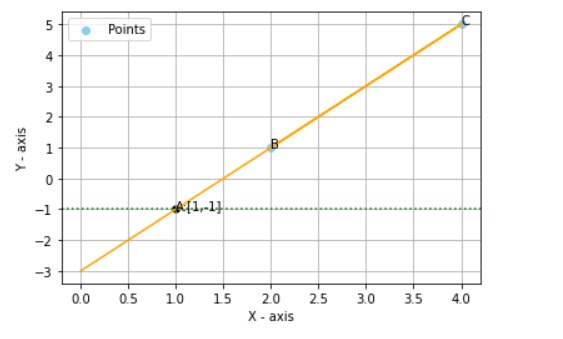
\includegraphics[width=\columnwidth]{solutions/aug/2/9/figures/figure.jpeg}
         \caption{Plot of the line }
         \label{aug/2/9/plot}
\end{figure}




\item Construct  right angled $\triangle $ whose hypotenuse  is 6 and one of the legs is 4.
\\
\solution

Let
\begin{align}
   \vec{A} = \myvec{2\\-1\\1} , \vec{B} = \myvec{1\\-3\\-5}, \vec{C} = \myvec{3\\-4\\-4} 
\end{align}

\begin{align}
     (\vec{B}-\vec{A})^\top(\vec{C}-\vec{A})&=\myvec{-1\ -2\ -6}\myvec{1\\-3\\-5}
     \\
& = 35 \ne 0
\\
     (\vec{A}-\vec{B})^\top(\vec{C}-\vec{B})&=\myvec{1\ 2\ 6}\myvec{2\\-1\\1}
\\
&= 6 \ne 0
\\
(\vec{A}-\vec{C})^\top(\vec{B}-\vec{C})&=\myvec{-1\ 3\ 5}\myvec{-2\\1\\-1}
\\
&= 0
\end{align}
Hence, $\triangle ABC$ is right angled at C as shown in Fig. \ref{aug/2/3plot}.
%
\begin{figure}[!h]
         \centering
         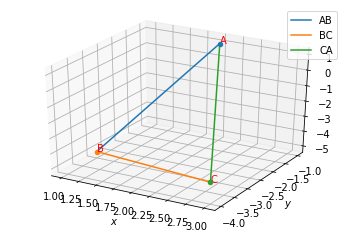
\includegraphics[width=\columnwidth]{solutions/aug/2/3/figures/right-angled.png}
         \caption{Plot of the triangle}
         \label{aug/2/3plot}
\end{figure}



\item Construct  an isosceles right angled $\triangle ABC$ right angled at $C$ such $AC = 6$.
\\
\solution
\input{solutions/26/ASSIGNMENT1.tex}

\item Construct $\triangle PQR$, given that $PQ = 3, QR = 5.5$ and $\angle PQR = 60 \degree$.
\\
\solution
\input{solutions/july/2/1/latex1.tex}
%
\item Construct $\triangle ABC$  with $BC = 7.5, AC = 5$ and $\angle C = 60\degree$.
\\
\solution
Let 
\begin{align}
    \vec{A}= \myvec{x\\-1} , \vec{B} = \myvec{2\\1} , \vec{C} = \myvec{4\\5}
\end{align}

Now,
\begin{align}
    \vec{B}-\vec{A} & = \myvec{2-x\\1-(-1)}\\
                    & = \myvec{2-x\\2}
\end{align}
\begin{align}
    \vec{B}-\vec{C} & = \myvec{2-4\\1-5}\\
                    & = \myvec{-2\\-4}
\end{align}

Forming the matrix $\vec{M}$,
\begin{align}
    \vec{M} & = \myvec{\vec{B}-\vec{A}  &  \vec{B}-\vec{C}}^\top \\
            & =\myvec{2-x & 2\\2 & -4}^\top\\
            & = \myvec{2-x & 2 \\ -2 & -4}
\end{align}

Using matrix transformation,


\begin{align}
 \vec{M} = \myvec{2-x & 2\\-2 & -4}
 \xleftrightarrow{\text{$R_2$}\rightarrow{\text{$R_2/2$}}} 
 \myvec{2-x & 2 \\-1 & -2}\\
 \xleftrightarrow{\text{$R_2$}\rightarrow{\text{$R_2 + R_1$}}}
 \myvec{2-x & 2 \\1-x & 0}
\end{align}
\begin{align}
 rank(\vec{M}) = 1 &\implies  R_2 =0 \\
 \text{or, }
            x=1
\end{align}
See Fig.          \ref{aug/2/9/plot}.
\begin{figure}[!h]
         \centering
         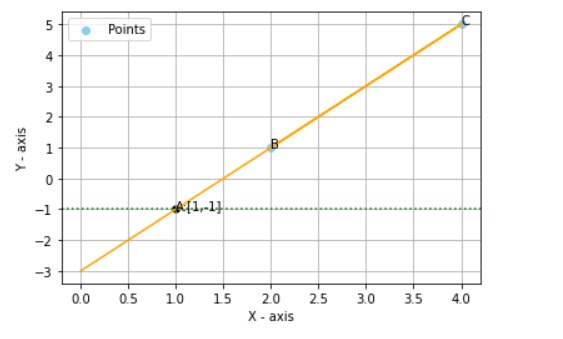
\includegraphics[width=\columnwidth]{solutions/aug/2/9/figures/figure.jpeg}
         \caption{Plot of the line }
         \label{aug/2/9/plot}
\end{figure}




\item Construct $\triangle XYZ$ if $XY = 6, \angle X = 30\degree$ and $\angle Y = 100 \degree$.
\\
\solution
\input{solutions/july/2/3/Latex.tex}

\item If $AC = 7, \angle A = 60\degree$ and $\angle B = 50 \degree$, can you draw the triangle?
%
\\
\solution
\input{solutions/july/2/4/assignment1.tex}

\item Construct $\triangle PQR$ if $PQ = 5, \angle Q = 105 \degree$ and $\angle R = 40 \degree$.
\\

Let the given Matrix be
\begin{equation}
\vec{A} = \myvec{3&5\\1&1}
\end{equation}
Transposing the above matrix gives,
\begin{equation}
\vec{A}^{\top} = \myvec{3&1\\5&1}
\end{equation}
Now, for Symmetric and Skew Symmetric Matrix,
\begin{align}
    \vec{B} &= \frac{\vec{A} + \vec{A}^{\top}}{2} = \myvec{3&3\\3&1} \\
    &= \vec{B}^{\top}
\end{align}
Also,
\begin{align}
    \vec{C} &= \frac{\vec{A} - \vec{A}^{\top}}{2} = \myvec{0&2\\-2&0} \\
    &= -\vec{C}^{\top}
\end{align}

Hence, $\vec{B}$ is a Symmetric Matrix and $\vec{C}$ is a Skew Symmetric Matrix and $\vec{B} + \vec{C} = \vec{A}$.
\begin{align}
    \therefore \myvec{3&5\\1&1} = \myvec{3&3\\3&1} + \myvec{0&2\\-2&0}  
\end{align}




\item Can you construct $\triangle DEF$ such that $EF = 7.2, \angle E = 110\degree$ and $\angle F = 180\degree$?



%\end{enumerate}

